% mnras_template.tex 
%
% LaTeX template for creating an MNRAS paper
%
% v3.0 released 14 May 2015
% (version numbers match those of mnras.cls)
%
% Copyright (C) Royal Astronomical Society 2015
% Authors:
% Keith T. Smith (Royal Astronomical Society)

% Change log
%
% v3.0 May 2015
%    Renamed to match the new package name
%    Version number matches mnras.cls
%    A few minor tweaks to wording
% v1.0 September 2013
%    Beta testing only - never publicly released
%    First version: a simple (ish) template for creating an MNRAS paper

%%%%%%%%%%%%%%%%%%%%%%%%%%%%%%%%%%%%%%%%%%%%%%%%%%
% Basic setup. Most papers should leave these options alone.
\documentclass[fleqn,usenatbib]{mnras}

% MNRAS is set in Times font. If you don't have this installed (most LaTeX
% installations will be fine) or prefer the old Computer Modern fonts, comment
% out the following line
% Depending on your LaTeX fonts installation, you might get better results with one of these:
% \usepackage{mathptmx}
% \usepackage{txfonts}

% Use vector fonts, so it zooms properly in on-screen viewing software
% Don't change these lines unless you know what you are doing
\usepackage[T1]{fontenc}

% Allow "Thomas van Noord" and "Simon de Laguarde" and alike to be sorted by "N" and "L" etc. in the bibliography.
% Write the name in the bibliography as "\VAN{Noord}{Van}{van} Noord, Thomas"
\DeclareRobustCommand{\VAN}[3]{#2}
\let\VANthebibliography\thebibliography
\def\thebibliography{\DeclareRobustCommand{\VAN}[3]{##3}\VANthebibliography}


%%%%% AUTHORS - PLACE YOUR OWN PACKAGES HERE %%%%%

% Only include extra packages if you really need them. Common packages are:
\usepackage{graphicx}	% Including figure files
\usepackage{amsmath}	% Advanced maths commands
\usepackage{amssymb}	% Extra maths symbols
\usepackage{newtxtext,newtxmath}

%%%%%%%%%%%%%%%%%%%%%%%%%%%%%%%%%%%%%%%%%%%%%%%%%%

%%%%% AUTHORS - PLACE YOUR OWN COMMANDS HERE %%%%%

% Packages for slightly better tables
\usepackage{booktabs}
% SI units package
\usepackage{siunitx} % Better units, especially SI
% Units used in work
\DeclareSIUnit[]\solarmass
{\text{\ensuremath{\textup{M}_{\odot}}}}
\DeclareSIUnit[]\solarluminosity
{\text{\ensuremath{\textup{L}_{\odot}}}}
\DeclareSIUnit[]\solarradius
{\text{\ensuremath{\textup{R}_{\odot}}}}
\DeclareSIUnit[]\year
{\text{yr}}
\DeclareSIUnit[]\au
{\text{AU}}
\DeclareSIUnit[]\parsec
{\text{pc}}
\DeclareSIUnit[]\erg
{\text{erg}}
\DeclareSIUnit[]\arcsecond
{\text{as}}

% Author commands
\newcommand{\ts}{\textsuperscript}

% Math macros 
\newcommand{\swr}{\ensuremath{_{\text{WR}}}}
\newcommand{\sob}{\ensuremath{_{\text{OB}}}}
\newcommand{\rms}[1]{\ensuremath{_{\text{#1}}}}
\newcommand{\mdot}{\dot{\text{M}}}
\newcommand{\dsep}{d\rms{sep}}

% Please keep new commands to a minimum, and use \newcommand not \def to avoid
% overwriting existing commands. Example:
%\newcommand{\pcm}{\,cm$^{-2}$}	% per cm-squared

%%%%%%%%%%%%%%%%%%%%%%%%%%%%%%%%%%%%%%%%%%%%%%%%%%

%%%%%%%%%%%%%%%%%%% TITLE PAGE %%%%%%%%%%%%%%%%%%%

% Title of the paper, and the short title which is used in the headers.
% Keep the title short and informative.
\title[Dust growth simulations of WR140]{Exploring dust growth in the episodic WCd system WR140}

% The list of authors, and the short list which is used in the headers.
% If you need two or more lines of authors, add an extra line using \newauthor
\author[J. W. Eatson, J. M. Pittard \& S. Van Loo]{
J. W. Eatson\thanks{E-mail: \href{mailto:py13je@leeds.ac.uk}{py13je@leeds.ac.uk}},
J. M. Pittard
and
S. Van Loo
\\
School of Physics and Astronomy, University of
       Leeds, Woodhouse Lane, Leeds LS2 9JT, UK\\  
}

% These dates will be filled out by the publisher
\date{Accepted XXX. Received YYY; in original form ZZZ}

% Enter the current year, for the copyright statements etc.
\pubyear{2022}

% Don't change these lines
\begin{document}
\label{firstpage}
\pagerange{\pageref{firstpage}--\pageref{lastpage}}
\maketitle

% Abstract of the paper
\begin{abstract}
\noindent


\end{abstract}

% Select between one and six entries from the list of approved keywords.
% Don't make up new ones.
\begin{keywords}
stars: Wolf-Rayet -- methods: numerical -- binaries: general
\end{keywords}

%%%%%%%%%%%%%%%%%%%%%%%%%%%%%%%%%%%%%%%%%%%%%%%%%%

%%%%%%%%%%%%%%%%% BODY OF PAPER %%%%%%%%%%%%%%%%%%

\section{Introduction}

% The dynamics of massive stars in binary systems is a particularly fascinating subject.
% These incredibly violent phenomena are obscured behind vast clouds of outflowing stellar wind, the result of the most massive stars we know slowly tearing themselves asunder.
Dust formation in massive star binary systems is a particularly fascinating subject.
Considering the immense photon fluxes and strong shocks involved, these systems should not form dust at all, and yet in some systems, all evidence points to the contrary.
% Observational history, define acronyms commonly used
Colliding wind binary (CWB) systems were first hypothesised to explain highly luminous and variable x-ray emission in systems such as V444 Cyg and $\gamma^2$ Vel \citep{prilutskii_x_1976}.
These extremely bright emissions were found to be due to stellar wind collision with shock velocities of the order $10^3 \, \si{\kilo\metre\per\second}$.
The variability in x-ray emission can be explained if the phenomena occurs due to the orbit of a binary system, such as the Wind Collision Region (WCR) being occluded by the outflowing stellar winds and being occluded by the stars themselves.
The system can also have an eccentric orbit, changing the shock strength as the orbital separation, $d\rms{sep}$, varies.
Despite this dust-hostile environment, CWB systems containing a Wolf-Rayet carbon phase star (WC) have been observed producing copious quantities of dust (so-called WCd systems).
These systems typically convert around $1\%$ of the stellar wind into dust a short time after wind collision; in more prolific systems such as WR104 up to $36\%$ of the Wolf-Rayet (WR) outflow is converted into dust \citep{lauRevisitingImpactDust2020}.
This corresponds to dust production rates on the order of $10^{-6} \, \si{\solarmass\per\year}$, rivalling other profuse dust producing phenomena such as AGB stars.

WCd systems can be sub-categorised further, into persistent, variable and episodic dust forming systems.
Persistent systems, such as WR104 \citep{tuthill_dusty_1999}, produce dust at a constant rate, and as such produce extreme quantities of dust, as well as well-defined pinwheel patterns if the system is viewed face-on.
Episodic systems, meanwhile, only produce dust for a limited period before entering a period of dormancy; this pattern is cyclical, and is predictably periodic.
A good example of such an episodic system is WR140 \citep{williamsMultifrequencyVariationsWolfrayet1990}, the subject of this paper.
Variable systems have some characteristics of these two sub-types, having a distinct variability without a period of dust producing dormancy, such as WR98a \citep{monnierPinwheelNebulaWR1999}.
Whether a system is persistent, variable or episodic is based on the system's orbital eccentricity.
Highly eccentric systems appear to form episodic systems, with the ``active'' dust production period occurring immediately after periastron passage, and a relatively short time thereafter.
Meanwhile, persistent and variable systems have been observed to have more circular orbits, suggesting that the effect of a change in system separation distance, $d\rms{sep}$, has a role in dust formation.
The initial mechanism behind dust formation is not well understood.
Whilst nascent amorphous carbon dust grain cores can condense within the photosphere of WC7-9 stars,
%%//TODO CITE THIS 
these grain cores would be vaporised by the UV flux of both stars.
However, within the WCR these grains appear to flourish.
Observations of these systems show that infrared excess in wavelengths associated with amorphous grains is detected almost exclusively within the post-shock WCR \citep{soulainSPHEREViewWolfRayet2018}.
% Dust forms close to system
Observations also indicate that dust formation occurs rapidly and close to the system, this requires strong radiative cooling for the immediate-post shock temperature to reduce from $\sim 10^7 \, \si{\kelvin}$ to $\sim 10^4 \, \si{\kelvin}$
\citep{williamsInfraredPhotometryLatetype1987,williamsMultifrequencyVariationsWolfrayet1990}.
% Bringing it all together, theories as to how dust formation occurs, density, shielding etc.
As such, dust formation appears to be encouraged in the WCR through a multitude of factors:

\begin{itemize}
  \item Strong radiative cooling produces clumps of cool, high density gas where dust can rapidly grow.
  \item The high density of the post-shock WCR results in a high collision rate between carbon atoms and dust grains.
  \item The high density also shields nascent dust grains from the bulk of the UV emission from the stars.
  \item The rapid cooling in the immediate post-shock environment reduces gas-grain sputtering.
\end{itemize}

\noindent
The dust formation can also be influenced by orbital separation, velocity shear and momentum ratio imbalance between the winds, producing variability on the timescale of a single orbit, or $t\rms{dyn} \ll P$.

\begin{table}
  \centering
  \resizebox{\linewidth}{!}{
  \begin{tabular}{lllllll}
    \hline
    & \multicolumn{2}{c}{Persistent} & \multicolumn{2}{c}{Variable} & \multicolumn{2}{c}{Episodic} \\ \cline{2-7} 
    & Total & Example & Total & Example & Total & Example \\ \hline
   WC4 & 1 & WR19 & 0 & --- & 0 & --- \\
   WC5 & 0 & --- & 0 & --- & 1 & WR47C \\
   WC6 & 1 & WR124-10 & 0 & --- & 0 & --- \\
   WC7 & 3 & WR102-22 & 0 & --- & 4 & WR140 \\
   WC8 & 6 & WR13 & 1 & WR48a & 3 & WR122-14 \\
   WC9 & 45 & WR104 & 6 & WR98a & 1 & WR75-11 \\ \hline
   Total & 56 &  & 7 &  & 9 &  \\ \hline
  \end{tabular}
  }
  \caption[Number of confirmed WCd systems]{Number of WCd systems with a known spectral type and dust formation type from the Galactic Wolf Rayet Catalogue \citep{rossloweSpatialDistributionGalactic2015}. Systems with uncertain spectral types are not included, while systems labelled ``d'' are included within the ``persistent'' category for their associated spectral type.}
  \label{tab:p2-wc-summated-list}
\end{table}

% Why not observe?
WCd systems are comparatively rare.
Out of 106 confirmed WR binaries, only 9 are categorised as episodic WCd systems
(Table \ref{tab:p2-wc-summated-list}).
As these systems have a typical distance on the order of $1-10 \, \si{\kilo\parsec}$, observation of WCds is difficult.
Whilst these systems can be observed and the dusty WCR can be resolved, observation of the innermost, immediate post-shock dust forming region is not possible at this distance.
As such, numerical simulation is necessary to determine dust formation in WCd systems.
A contemporary example of such simulations is \cite{hendrix_pinwheels_2016}, though the evolution of dust grains through cooling, growth and sputtering was not performed.
% What we intend to do in this project
In this paper we present a numerical simulation of the archetypical episodic WCd system WR140 with a co-moving dust model simulating grain growth and sputtering through gas-grain collisions.
This simulation covers a temporal slice of the orbit of WR140 from phase $\Phi = 0.95$ to $\Phi = 1.10$, or the period immediately prior to and after periastron passage.
We will discuss our methodology in Section \ref{sec:paper-2-methodology}, with a particular emphasis on our dust model in Subsection \ref{sec:dust-model}.
Afterwards we will discuss the simulation and WR140 system parameters, as well as our data collection techniques in Section \ref{sec:paper2-wr140}.
Finally, we will discuss our results and conclude in Sections \ref{sec:p2-results} and \ref{sec:p2-conclusion}.

\section{Methodology}
\label{sec:paper-2-methodology}

The periodic dust forming system WR140 was simulated using a fork of the Athena++ hydrodynamical code \citep{stoneAthenaAdaptiveMesh2020}.
A series of modifications were implemented to simulate binary system orbits, stellar wind outflows and dust evolution.
These simulations were conducted in 3D in a Cartesian co-ordinate system.
The code solves a Riemann problem at each cell interface to determine the time-averaged values at the zone interfaces, and then solves the equations of hydrodynamics:

\begin{subequations}
  \begin{align}
    \frac{\partial\rho}{\partial t} & +\nabla \cdot \left(\rho \boldsymbol{u}\right) = 0 , \\
    \frac{\partial \rho \boldsymbol{u}}{\partial t} & + \nabla \cdot \left(\rho \boldsymbol{u} u + P \right) = 0, \\
    \frac{\partial \rho \varepsilon}{\partial t} & + \nabla \cdot \left[ \boldsymbol{u} \left( \rho\varepsilon + P \right) \right] = \frac{dE\rms{cool}}{dt} , 
  \end{align}
\end{subequations}

\noindent
where $\varepsilon$ is the total specific energy ($\varepsilon = \boldsymbol{u}^2/2 + e/\rho $), $\rho$ is the gas density, $e$ is the internal energy density, $P$ is the gas pressure and $u$ is the gas velocity.
In order to simulate radiative losses, the parameter $dE_\text{cool}/dt$ is included, which is the energy loss rate per unit volume from the fluid due to gas and dust cooling.

Spatial reconstruction using a piecewise linear method was performed, while two strong stability Runge-Kutta methods were used for numerical integration, depending on the simulation stability.
Several passive scalars are utilised to model wind mixing and dust evolution, which are transported by the fluid.
For a given scalar, $i$, the scalar is advected through the following equation:

% \begin{equation}
%   \rho \frac{dC_i}{dt} = \frac{\partial}{\partial t} \left( \rho C_i \right) + \nabla \cdot \left( C_i \rho \mathbf{u} \right) = -\nabla \cdot \mathbf{Q}_i ,  
% \end{equation}

\begin{equation}
  \rho \frac{dC_i}{dt} = \frac{\partial}{\partial t} \left( \rho C_i \right) + \nabla \cdot \left( C_i \rho \mathbf{u} \right) = 0 ,  
\end{equation}

\noindent
where $C_i$ is the scalar quantity.
Passive scalar diffusion is set to 0, hence the scalars are explicitly co-moving with the fluid. %\citep{stoneAthenaAdaptiveMesh2020}.

% Cover mapping on winds

Stellar winds are simulated by modifying the density, $\rho_R$, momentum, $p_R$, and energy, $E_R$ in a small region around both stars.
Winds flow from this ``remap'' region at the stars wind terminal velocity, $v^\infty$. Remap zone parameters are calculated with the formulae

\begin{subequations}
  \begin{align}
    \rho_R & = \frac{\mdot}{4 \pi r^2 v_\infty} , \\
    % P_R    & = \frac{\rho_R}{\mu m_H} k_B T_w , \\
    p_R    & = \rho_R v_{r} , \\
    E_R    & = \frac{P_R}{\gamma - 1} + \frac{1}{2} \rho_R v_\infty^2 ,
  \end{align}
\end{subequations}

\noindent
where $P_R$ is the cell pressure ($P_R = \rho_R k_\text{B} T_w / \mu m_\text{H}$), $T_w$ is the wind temperature, $\mu$ is the mean molecular mass, $m_\text{H}$ is the mass of a hydrogen atom, $v_R$ is the wind velocity as it flows radially from the center of the ``remap zone'' and $r$ is the distance from the current cell to the centre of the remap zone.
This method produces radially out-flowing winds from the star with an expected density and velocity.
% This method is stable against numerical instability, while also allowing us to precisely control the winds.

Line driving and wind acceleration effects are not simulated;
% , which can result in divergence with the correct wind velocity as stars approach periastron passage.
instead, winds are instantaneously accelerated to their terminal velocity.
% Additionally, influence on the fluid from either gravitational self-interaction or interaction with the stars gravity wells are not simulated, with the stellar winds assumed to be travelling far in excess of the system escape velocity.
Gravitational forces are not calculated as the winds are assumed to be travelling in excess of the system escape velocity.

Athena++ utilises Message Passing Interface (MPI) parallelism.
The numerical problem is broken into blocks, which are distributed between processing nodes on a High Performance Compute (HPC) cluster.
The block size is variable, but for this simulation a block size of $40\times 40 \times 10$ cells in $XYZ$ was found to be optimal.
% Adaptive Mesh Refinement was considered for this simulation, however a known issue with the Athena++ code prevented this from being possible.
% Passive scalars incorporated into the simulation were found to not be conserved along the interfaces between mesh blocks undergoing refinement, this meant that the simulation would rapidly exhibit unphysical behaviour (this bug is recorded as issue \#365 on the Athena++ Github repository\footnote{\texttt{\href{https://github.com/PrincetonUniversity/athena/issues/365.}{https://github.com/PrincetonUniversity/athena/issues/365}}}).
% A ring of refined cells across the orbital path was considered, but the performance improvements of this method were found to be negligible and not worth pursuing, as the block based refinement method of Athena++ would result in significant redundant refinement.
% Instead, a static mesh is used, where the stars predicted orbit over the simulation is refined to the maximum level, with a gradual de-refinement away from this refinement region.
Static mesh refinement is used to increase the effective resolution of the simulation.
A region around the orbital path of the stars in the simulation is refined to a higher resolution, with gradual de-refinement as a function of distance from this refinement region.
This refinement is covered in more detail in Section \ref{sec:p2-sysparameters}.

\subsection{Radiative cooling}

Cooling is simulated via the removal of thermal energy from a cell at each time-step.
A cooling rate, for radiative emission from the stellar wind gas, $dE\rms{g}/dt$, is calculated and integrated using a sub-stepping Euler method.
The number of sub-steps is determined by the estimated cooling timescale of the cell.
Cooling is calculated via individual lookup tables from each wind.
These lookup tables contain the normalised emissivity, $\Lambda\rms{w}(T)$ at a logarithmically spaced series of temperatures from $10^4 \, \si{\kelvin}$ to $10^9 \, \si{\kelvin}$.
The cooling rate is determined for a cell by calculating the cell temperature and estimating $\Lambda\rms{w}(T)$ using linear interpolation between the nearest emissivity values in the lookup table.
The energy loss is then calculated through the equation:

\begin{equation}
  \frac{dE\rms{g}}{dt} = \left(\frac{\rho\rms{g}}{m\rms{H}}\right)^2 \Lambda\rms{w}(T),
\end{equation}

\noindent
where $\rho\rms{g}$ is the gas density and $m\rms{H}$ is the mass of hydrogen.
The lookup table was generated by mixing a series of cooling curves from MEKAL calculation of elemental gasses.
These curves were combined based on the elemental abundances in the WC and OB winds.
To save calculation time, temperatures between $\SI{1e4}{\kelvin} < T \leq \SI{1.1e4}{\kelvin}$ are set to \SI{1e4}{\kelvin} as they are assumed to be either rapidly cooling or a part of the stellar wind outside of the WCR.
A minimum temperature of $10^4 \, \si{\kelvin}$ is defined by the simulation, is it is assumed that a radiating post-shock wind will tend to the temperature of the pre-shock wind, $T\rms{final} \rightarrow T\rms{pre-shock}$.

\subsection{Dust model}
\label{sec:dust-model}

In order to simulate dust evolution in WR140 a passive scalar dust model that simulates dust growth and destruction is included in the simulation.
The dust model operates on passive scalars, and as such simulates dust that is co-moving with the stellar wind.
Two scalars are used to describe dust in a cell, $a$, the grain radius in microns, and $z$, the grain dust-to-gas mass ratio

\begin{equation}
  z = \frac{\rho\rms{d}}{\rho\rms{g}},
\end{equation}

\noindent
where $\rho\rms{d}$ is the dust density in the cell.
A number of assumptions are made in this dust model; for instance, the dust grains in the model are spherical, with a uniform density.
Dust grains are assumed to have a single size each grid cell.
The number density of grains varies in the simulation volume, however the ratio of grain number density is fixed and constant throughout the simulation.
As such, this model does not simulate grain fracturing.
Additional mechanisms for dust formation and destruction could also be implemented such as grain-grain agglomeration and photoevaporation.
A multi-fluid model with drag force coupling could also be implemented, however this is beyond the scope of this paper.

Dust grows through grain accretion using formulae described by \cite{spitzer_jr._physical_2008} where dust grains grow via low-velocity collisions with surrounding carbon atoms, causing them to accrete onto the surface of the dust grain.
Carbon is removed from the gas, reducing the cell gas density, while the corresponding dust density increases.
This ensures that mass is preserved in the simulation.
Assuming a single average grain size the rate of change in the grain radius in a cell, $da/dt$, is given by the equation:

\begin{equation}
  \frac{da}{dt} = \frac{\xi \rho\rms{C} w\rms{C}}{4\rho\rms{gr}},
\end{equation}

\noindent
where $\xi$ is the grain sticking factor, $\rho\rms{C}$ is the carbon density ($\rho\rms{C} = X\rms{C} \rho\rms{g}$), $w\rms{C}$ is the Maxwell-Boltzmann RMS velocity for carbon ($w\rms{C} = \sqrt{3k\rms{B} T / 12m\rms{H}}$), $k\rms{B}$ is the Boltzmann constant and $\rho\rms{gr}$ is the grain bulk density.
The rate of change in the mass of a single grain due to accretion, $dm\rms{gr,ac}/dt$, is calculated with the formulae:

\begin{equation}
  \frac{d m\rms{gr,acc}}{dt} = 4 \pi \rho\rms{gr} a^2 \frac{da}{dt} = \pi \xi \rho\rms{C} w\rms{C} a^2, \\
\end{equation}

\noindent
A bulk density approximating that of amorphous carbon grains ($\rho\rms{gr} = \SI{3.0}{\gram\per\centi\metre\cubed}$) is used for this simulation.

Dust destruction through gas-grain sputtering is calculated using the \cite{drainePhysicsDustGrains1979} prescription.
Within a flow of gas number density $n\rms{g}$ a dust grain of radius $a$ has a grain lifespan, $\tau\rms{gr}$ of:

\begin{equation}
  \tau\rms{gr} = \frac{a}{\dot{a}} \approx \num{3e6} \frac{a}{n\rms{g}} \, \si{\year} .
\end{equation}

\noindent
This value is based on an average lifetime of carbon grains in an interstellar shock with a temperature of $\SI{1e6}{\kelvin} \leq T \leq \SI{3e8}{\kelvin}$ \citep{tielens_physics_1994,dwekCoolingSputteringInfrared1996}.
The rate of change in the mass of a single dust grain due to sputtering, $dm\rms{gr,sp}/dt$, can then be calculated with a similar formula to the rate of change in grain mass due to accretion:

\begin{equation}
  \frac{d m\rms{gr,sp}}{dt} = -4 \pi \frac{\rho\rms{gr} a^3}{\tau\rms{d}} = -4\pi \frac{\rho\rms{gr} n\rms{g} a^2}{\num{3e6}}
\end{equation}

\noindent
The overall change in dust density is then calculated through the equation:

\begin{equation}
  \frac{d \rho\rms{d}}{dt} = \left( \frac{d m\rms{gr,acc}}{dt} + \frac{d m\rms{gr,sp}}{dt}\right) n\rms{d}, 
\end{equation}

\noindent
where $n\rms{d}$ is the dust grain number density.

Cooling via emission of photons from dust grains is also included in this model.
The rate of cooling is calculated using the uncharged grain case of the prescription described in \cite{dwek_infrared_1981}.
Grains are collisionally excited by collisions with ions and electrons, causing them to radiate.
Similarly to the gas/plasma emission model used, the emitted photons are not re-adsorbed by the WCR medium, causing energy to be removed from the simulation.
This therefore makes the assumption that the WCR is optically thin to far-infrared photons, which is observationally correct \citep{monnierKeckAperturemaskingExperiment2007,soulainSPHEREViewWolfRayet2018,callinghamAnisotropicWindsWolf2019}.
The grain heating rate, $H\rms{coll}$, in \si{\erg\per\second} for a dust grain is calculated with the formulae:

\begin{equation}
  \label{eq:p2-grainheat}
  H = 1.26 \times 10^{-19} \frac{n\rms{g}}{A^{1/2}} a^2(\si{\micro\metre}) T^{3/2} h(a,T) , 
\end{equation}

\noindent
% where $H$ is the heating rate due to atom and ion collisions, 
where $n\rms{g}$ is the gas number density,
$A$ is the mass of the incident particle in AMU,
$a(\si{\micro\metre})$ is the grain radius in microns,
$T$ is the temperature of the ambient gas,
and $h(a,T)$ is the effective grain heating factor.
Individual heating rates for hydrogen, helium, carbon, nitrogen and oxygen are calculated, in order to calculate the total ion collisional heating, $H\rms{coll}$:

\begin{equation}
  H\rms{coll} = H\rms H + H \rms{He} + H\rms C + H\rms N + H\rms O .
\end{equation}

\noindent
The effective grain heating factor for each element is calculated via the equation:

\begin{equation}
  h(a,T) = 1 - \left( 1 + \frac{E^*}{2 k\rms{B} T} \right) e^{- E^* / k\rms{B} T} ,
\end{equation}

\noindent
where $E^*$ is the critical energy required for the particle to penetrate the dust grain (Table \ref{tab:p2-criticalenergy}).
The rate of heating due to electron-grain collisions, $H\rms{el}$, is similar to Eq. \ref{eq:p2-grainheat}.
The grain heating factor for electron collisions, $h\rms{e}$, is calculated via an approximation rather than the exact calculation in the case of baryonic matter.
% This approximation is performed as a complex integration for every cell and cooling step would need to be performed instead, which was found to take up $>90\%$ of the processing time per cell.
$h\rms{e}$ is estimated through the following conditions:

\begin{equation}
  \begin{alignedat}{3}
    h\rms{e}(x^*) & = 1 ,                && ~~ x^* > 4.5, \\
             & = 0.37{x^*}^{0.62} , && ~~ x^* > 1.5 , \\
             & = 0.27{x^*}^{1.50} , && ~~ \text{otherwise,}
  \end{alignedat}
\end{equation}

\noindent
where $x^* = \num{2.71e8} a^{2/3} (\si{\micro\metre})/T$.
This approximation differs from the integration method by less than 8\% while being 3 orders of magnitude faster.
Excitation due to grain-grain collisions were not modelled, due to the limitations of the passive scalar model.
In order to calculate the change in energy due to dust cooling, we find the radiative emissivity for dust, $\Lambda\rms{d}(T,a)$, to be

\begin{equation}
  \Lambda(T,a) = \frac{H\rms{coll} + H\rms{el}}{n\rms{H}} ,
\end{equation}

\noindent
where $n\rms{H}$ is the number density of hydrogen in the gas.
The energy loss rate from dust cooling, $dE\rms{d}/dt$, then calculated with the equation:

\begin{equation}
  \frac{dE\rms{d}}{dt} = n\rms{T} n\rms{d} \Lambda\rms{d} (T,a) , 
\end{equation}

\noindent
and added to the gas/plasma energy loss rate, such that the total energy loss rate is:

\begin{equation}
  \frac{dE\rms{cool}}{dt} = \frac{dE\rms{g}}{dt} + \frac{dE\rms{d}}{dt} .
\end{equation}

\begin{table}
  \centering
  \begin{tabular}{ll}
    \hline
    Particle & $E^*$ \\
    \hline
    $e^-$ & $23 \, a^{2/3}(\si{\micro\metre})$ \\
    H     & $133 \, a(\si{\micro\metre})$ \\
    He    & $222 \, a(\si{\micro\metre})$ \\
    C     & $665 \, a(\si{\micro\metre})$ \\
    N     & $665 \, a(\si{\micro\metre})$ \\
    O     & $665 \, a(\si{\micro\metre})$ \\
    \hline
  \end{tabular}
  \caption[Grain critical energy]{Grain critical energy, $E^*$, for a dust grain of $a$ in \si{\micro\metre} for electrons, $e^-$, as well as the elements considered for grain cooling. The values for carbon, oxygen and nitrogen are identical.}
  \label{tab:p2-criticalenergy}
\end{table}

\section{System parameters}
\label{sec:paper2-wr140}

We have previously simulated WCd systems in the form of a parameter space exploration, in order to discern which wind and orbital parameters are influential on the dust growth rates \textcolor{red}{\underline{\emph{\textbf{CITE EATSON ET AL. 2022 WHEN PUBLISHED}}}}.
%\cite my own damn work
It was determined that the primary factors of dust growth in a WCd system were the mass loss rates, $\mdot$, and wind terminal velocities, $v^\infty$, for each star, as well as the orbital separation, $d\rms{sep}$.
In particular, it was found that imbalances between the wind velocity produced Kelvin-Helmholtz (KH) instabilities due to a shear in the winds.
Slower winds were found to be more radiative in the post-shock WCR flow, cooling to temperatures suitable for dust formation.
This was found to influence the dust growth rate by as much as six orders of magnitude through a factor of four variation of the WR wind terminal velocity.
We also found that increasing $d\rms{sep}$ significantly reduced the dust production rate, due to less intensive shocks as the out-flowing winds became less dense with distance.
In the case of WCd systems with eccentric orbits, the separation distance can vary significantly.
In the case of WR140, $\dsep$ varies by a factor of 18 from apastron to periastron.
This is hypothesised to be the primary cause of dust production variability within episodic systems.
% As $\mdot$ does not vary significantly on the orbital timescale of these systems, this is not expected to impact the dust growth rate in episodic systems, while the wind velocity can diverge somewhat due to radiative inhibition and orbital motion.
The pre-shock velocity can also vary somewhat due to radiative inhibition and orbital motion.
%  which was considered in our results.

In order to understand the structure and dynamics of the CWB system we must define some important parameters, such as the wind momentum ratio, $\eta$, which is defined as:

\begin{equation}
  \eta = \frac{\mdot\sob v^\infty\sob}{\mdot\swr v^\infty\swr} .
\end{equation}

\noindent
As $\eta$ decreases we find that the wind becomes more imbalanced.
In the case of WR+OB CWB systems we find that the WR stars wind typically dominates the WCR.
% Assuming that there is no radiative inhibition \citep{stevens_stagnation-point_1994} or radiative braking \citep{gayley_sudden_1997},
% the distance from each star to the apex of the WCR can be estimated using $\eta$:
% \begin{subequations}
%   \begin{align}
%     r\rms{WR} & = \frac{1}{1 + \eta^{1/2}} d\rms{sep}, \\
%     r\rms{OB} & = \frac{\eta^{1/2}}{1 + \eta^{1/2}} d\rms{sep} ,
%   \end{align}
% \end{subequations}
% \noindent
% where $r\rms{WR}$ is the distance from the WR star to the WCR apex and $r\rms{OB}$ is the distance from the OB star to the WCR apex.
Assuming that there is no radiative inhibition \citep{stevens_stagnation-point_1994} or radiative braking \citep{gayley_sudden_1997}, we can approximate the WCR to a conical region with an opening angle:

\begin{equation}
  \theta\rms{c} \simeq 2.1 \left( 1 - \frac{\eta^{2/5}}{4}\right) \eta^{-1/3} ~~~ \text{for} ~ 10^{-4} \leq \eta \leq 1 ,
\end{equation}

\noindent
to a relatively high degree of accuracy \citep{eichler_particle_1993}.
Another important value for determining the nature of the WCR is the cooling parameter, $\chi$, which is the ratio of the time taken for the shocked wind to completely cool to the time taken for the wind to escape the shocked region:

\begin{equation}
  \label{eq:p2-chi}
  \chi = \frac{t_\text{cool}}{t_\text{esc}} \approx \frac{v_{8}^4 d_{12}}{\dot{\text M}_{-7}} , 
\end{equation}

\noindent
where $v_{8}$ is the wind terminal velocity in units of $10^8 \, \si{\centi\metre\per\second}$, $d_{12}$ is the separation distance in units of $10^{12} \, \si{\centi\metre}$ and $\mdot_{-7}$ is the wind mass loss rate in units of $10^{-7} \, \si{\solarmass\per\year}$ \citep{stevens_colliding_1992}.
As $\chi$ decreases, the structure of the WCR becomes more influenced by cooling.
% by radiative instabilities, and has a post-shock temperature approaching the initial wind temperature.
If $\chi < 1$, the WCR is completely dominated by radiative cooling, while if $\chi \gg 1$, the WCR behaves adiabatically.
If the WCR is highly radiative the total compression can be significantly greater than the adiabatic limit of 4 for a $\gamma = 5/3$ gas, which facilitates dust production.
Finally, we define a maximum dust production rate of the system, $\mdot\rms{d,max}$, assuming a 100\% conversion rate of WR wind in the WCR into dust.
The fraction of the WR wind that is passed through the WCR is given by the equation:

\begin{equation}
  f\rms{WR} = \frac{1 - \cos\left(\theta\rms{WR}\right)}{2},
\end{equation}

\noindent
where $\theta\rms{WR}$ is the opening angle of the WR shock front ($\theta\rms{WR} \approx 2 \tan^{-1}(\eta^{1/3}) + \pi/9$, see \cite{pittardCollidingStellarWinds2018}).
$\mdot\rms{d,max}$ is then calculated with the formulae:

\begin{equation}
  \label{eq:p2-maxdustrate}
  \mdot\rms{d,max} = \mdot\rms{WR} X\rms{C,WR} f\rms{WR},
\end{equation}

\noindent
where $X\rms{C,WR}$ is the carbon mass fraction in the WR star.

\subsection{WR140 parameters}

% Discuss importance of WR 140 system
WR140 was simulated in this paper as it is an archetypical example of an episodic WCd system.
The system has an extremely eccentric orbit, which significantly affects the cooling parameter as the orbit progresses, and is also observed in detail.
% Additionally, the minimum value for $\chi$ is significantly larger than the other systems, and hence cooling would be less dominant on the dynamics of the WCR, even at periapsis.
% Though this simulation does not calculate wind acceleration due to radiative line driving,
Both stellar winds are expected to be accelerated to close to their terminal wind velocities before they collide \citep{lamersIntroductionStellarWinds1999}.
% However, this discrepancy should be noted when considering the results of this paper.

% Discuss simulation parameters
Recent improved estimations of the orbital parameters of WR140 by \cite{thomasOrbitStellarMasses2021} were used to calculate the orbit for these simulations, while the mass loss rate, and the wind terminal velocity were taken from \cite{williamsMultifrequencyVariationsWolfrayet1990}
(see Table \ref{tab:wr140systemparameters}).
% Composition
% In order to correctly calculate cooling and dust growth, the abundances of hydrogen, helium, and metals, particularly CNO must be included in the simulations parameters.
A typical wind composition for WC stars was assumed for the Wolf-Rayet star, while a solar abundance was assumed for the OB star (Table \ref{tab:p2-abundances}).
% The system orbit was calculated using a Keplerian orbital model with the two stars as point-masses.
% Self-gravity of the winds were not considered, as the winds leave the numerical grid quickly, and are travelling at a terminal velocity far in excess of the wind escape velocity, $v^\infty \gg v\rms{esc}$.

\begin{table}
  \centering
  \begin{tabular}{lll}
    \hline
    Parameter & Value & Citation \\
    \hline
    $\text{M}_\text{WR}$ & \SI{10.31}{\solarmass} & \cite{thomasOrbitStellarMasses2021} \\
    $\text{M}_\text{OB}$ & \SI{29.27}{\solarmass} & \cite{thomasOrbitStellarMasses2021} \\
    $P$ & \SI{7.926}{\year} & \cite{thomasOrbitStellarMasses2021} \\
    $e$ & 0.8993 & \cite{thomasOrbitStellarMasses2021} \\
    $\dot{\text{M}}_\text{WR}$ & \SI{5.6e-5}{\solarmass\per\year} & \cite{williamsMultifrequencyVariationsWolfrayet1990} \\
    $\dot{\text{M}}_\text{OB}$ & \SI{1.6e-6}{\solarmass\per\year} & \cite{williamsMultifrequencyVariationsWolfrayet1990} \\
    $v^\infty_\text{WR}$ & \SI{2.86e3}{\kilo\metre\per\second} & \cite{williamsMultifrequencyVariationsWolfrayet1990} \\
    $v^\infty_\text{OB}$ & \SI{3.20e3}{\kilo\metre\per\second} & \cite{williamsMultifrequencyVariationsWolfrayet1990} \\
    $\eta$ & 0.031 & Calculated \\
    $\chi_\text{min}$ & 2.69 & Calculated \\
    \hline
  \end{tabular}
  \caption[WR140 system parameters]{The system parameters for the WR140 system as used in this paper. References for each parameter are provided.}
  \label{tab:wr140systemparameters}
\end{table}

\begin{table}
  \centering
  \begin{tabular}{lll}
  \hline
  Element & Solar & WC \\ \hline
  $X\rms H   $ & $0.705$ & $0.000$ \\
  $X\rms{He} $ & $0.275$ & $0.546$ \\
  $X\rms C   $ & $0.003$ & $0.400$ \\
  $X\rms N   $ & $0.001$ & $0.000$ \\
  $X\rms O   $ & $0.010$ & $0.050$ \\
  \hline
  \end{tabular}
  \caption[Abundances by mass used for OB and WR stars]{Abundances used for the OB and WR stars being simulated. Other elements are assumed to be trace when calculating dust emission \citep{williamsSpectraWC9Stars2015}.}
  \label{tab:p2-abundances}
\end{table}

\subsection{Simulation parameters}
\label{sec:p2-sysparameters}

% Discuss more simulation parameters

A domain of $128 \times 128 \times 16 \, \si{\au}$ was used for this simulation, with a coarse (0\ts{th} level) grid resolution of $400\times 400 \times 50$ cells in the XYZ domain.
The simulation has 4 refinement levels, corresponding to an effective resolution of $6400 \times 6400 \times 800$ cells and a cell size of $0.02^3 \, \si{\au\cubed}$.
At periastron passage this results in $\sim 80$ cells between the stars, which was found to be enough to adequately resolve the WCR. 
This simulation has an XYZ aspect ratio of 8:8:1 in order to reduce processing time, as the bulk of dust formation was expected to occur a short distance from the WCR.
% Due to computing limitations, a complete orbit could not be completed without AMR, instead,
A section of the systems orbit, corresponding to an orbital phase of $0.95 \leq \Phi \leq 1.10$ was simulated (Fig. \ref{fig:p2-trajectory}).
This represents \num{1.2} year section of the systems orbit, and is the orbital period where much of the dust forms - prior to and shortly after periastron passage \citep{crowther_dust_2003}.
Fig. \ref{fig:p2-orbitalpath} shows the orbit overlaid onto the statically refined numerical grid.
The area of maximum refinement is around the orbital paths of the stars from $0.94 \leq \Phi \leq 1.11$, in order to ensure that the stars and the apex of the WCR are maximally refined.
% If the stars leave the regions that are refined to either the 3\ts{rd} or 4\ts{th} level unphysical behaviour with regards to wind mapping and dust formation occur, as such the simulation is halted when $\Phi = 1.10$.
The simulation was run with two different numerical integrators, a 3\ts{rd} order accurate Runge-Kutta integrator, \texttt{rk3}, and a 4\ts{th} order accurate, 5-stage, 3 storage register strong stability preserving Runge-Kutta integrator, \texttt{ssprk5\_4}
\citep{ruuthHighOrderStrongStabilityPreservingRungeKutta2005}.
The \texttt{ssprk5\_4} integrator was found to be approximately 60\% slower, but markedly more stable.
Prior to periastron passage the \texttt{rk3} integrator was used for its speed, but increasing numerical instability as the stars grew closer resulted in this proving untenable, and it was switched to \texttt{ssprk5\_4} for the remainder of the simulation.

During periastron passage the average time-step was found to reduce by an order of magnitude, resulting in a corresponding increase to simulation time. %(Fig. \ref{fig:p2-timestep}).
At the most numerically complex portion of the simulation, a Courant number of $C = 0.04$ had to be used instead of the initial value of $C = 0.15$, in order to preserve numerical stability.
As the simulation moved past periastron the Courant number was increased every 24 hours of wall time, until $C$ returned to the initial value.
The simulation was conducted on the ARC4 HPC cluster at the University of Leeds with 128 cores.
The code was compiled using the Intel \texttt{ICPC} compiler using \texttt{AVX512} optimisations and the Intel MPI library.

\begin{figure}
  \centering
  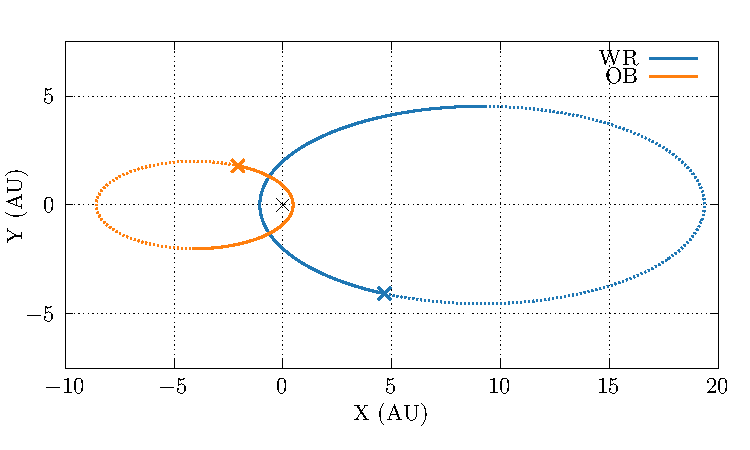
\includegraphics[width=\linewidth]{assets/trajectory/wr140-orbit.pdf}
  \caption[Orbital trajectories of WR140 WC7 and O5 stars]{Orbital trajectories of the WC7 and O5 stars in WR140. The solid lines represent the orbital phase being simulated, corresponding to $0.95 \leq \Phi \leq 1.10$, while the dashed lines represent the full orbital trajectory. The starting position for each star and the orbital barycentre at (0,0) are annotated.}
  \label{fig:p2-trajectory}
\end{figure}

\begin{figure}
  \centering
  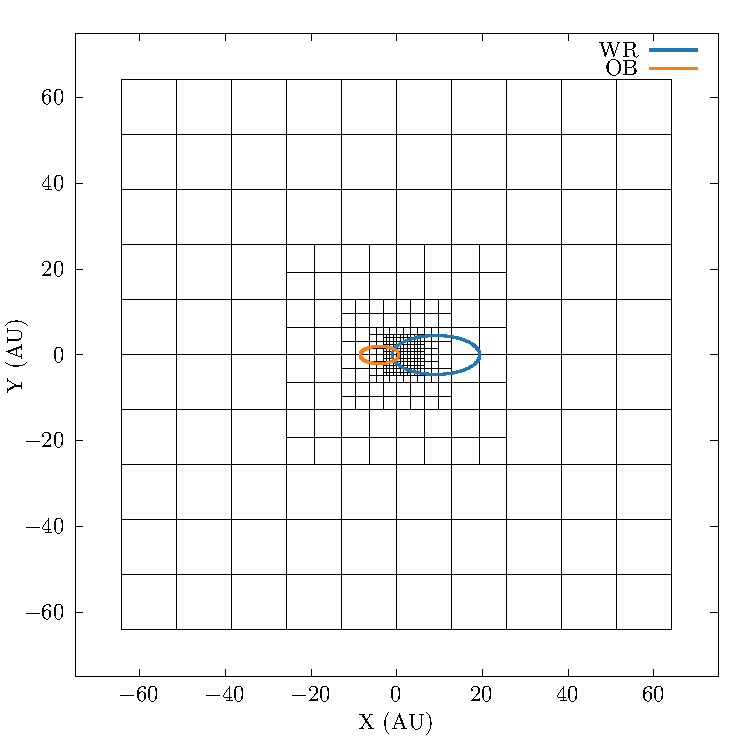
\includegraphics[width=\linewidth]{assets/wr140-grid/grid-orbit.pdf}
  \caption[Numerical grid of the WR140 system simulation at $z=0$]{Numerical grid of the WR140 system simulation at $z=0$. Static mesh refinement was used to increase the resolution around the orbital path from $0.95 \leq \Phi \leq 1.10$. The orbital path of both stars are overlaid onto this numerical grid. The stars are typically in the 3\ts{rd} or 4\ts{th} level.}
  \label{fig:p2-orbitalpath}
\end{figure}

% \begin{figure}
%   \centering
%   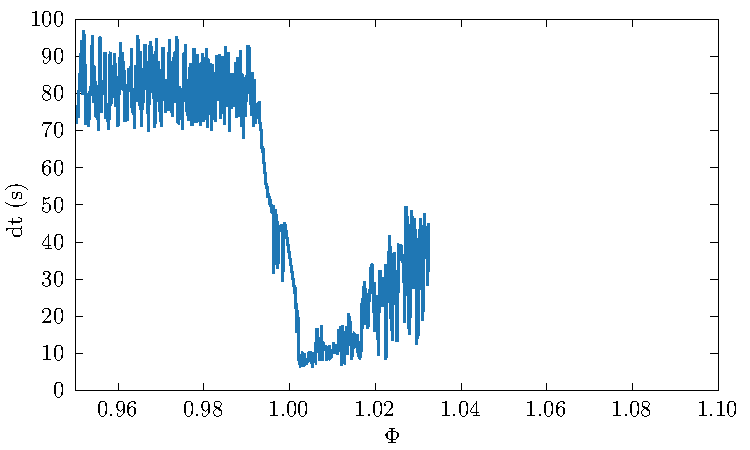
\includegraphics[width=\linewidth]{assets/wr140-dt.pdf}
%   \caption[Timestep over WR140 simulation]{Average timestep, $dt$, over the course of the WR140 simulation, binned every $\Phi = 0.001$. after periastron passage the \texttt{ssprk5\_4} numerical integrator and a drastically reduced Courant number was adopted in order to preserve numerical stability. This increased simulation time by approximately an order of magnitude.}
%   \label{fig:p2-timestep}
% \end{figure}

\subsection{Data collection}
% Data collection 
Simulation data was exported as HDF5 files at regular time intervals.
3D meshes were collected every increment of $\delta \Phi = \num{1.5e-3}$, while 2D slices in the XY plane were collected every increment of $\delta \Phi = \num{1.5e-4}$.
These HDF5 files contain the primitive variables of the simulation: gas density, $\rho$, gas pressure, $P$, and wind velocity components, $v_x$, $v_y$ and $v_z$.
These variables were then used to derive other variables such as temperature and energy.
The scalars governing the dust properties were also stored for each cell: the dust-to-gas mass ratio, $z$, and the dust grain radius, $a$.
The wind ``colour'', the proportion of gas from each star, was also stored.
A value of 1.0 indicates a pure WR wind while 0.0 indicates a pure OB wind.
The volume-weighted totals of all parameters of interest were also collected, such as the average values for $z$, $a$ and the dust production rate within the WCR, $\dot{\text{M}}\rms{d}$.
To calculate $\dot{\text{M}}\rms{d}$, a cell must be identified as being within the WCR.
This was performed by comparing the cell density to the predicted density of a single wind with the wind parameters of the WC star in the system.
Any cell with a density higher than a certain threshold value was flagged as being within the WCR.
The single-wind density, $\rho\rms{SW}$, was calculated using the equation:

\begin{equation}
  \rho\rms{SW} = \frac{\dot{\text{M}}\rms{SW}}{4\pi r^2 v^\infty\rms{SW}},
\end{equation}

\noindent
where $r$ is the distance from the barycentre.
This threshold value was set to $\rho\rms{thres} = 1.25\rho\rms{SW}$, which was found to accurately identify the WCR through thorough prior testing.

\section{Results}
\label{sec:p2-results}

% Dust production rate

\begin{table}
  \centering
  \begin{tabular}{lll}
  \hline
  Parameter & Mean & Maximum \\ \hline
  $\dot{\text{M}}\rms{d}$ (\si{\solarmass\per\year}) & \num{7.68e-08} & \num{1.24e-06} \\
  $\bar{a}$ (\si{\micro\metre}) & \num{1.32e-02} & \num{1.44e-02} \\
  $\bar{z}$ & \num{3.98e-04} & \num{3.32e-03} \\ \hline
  \end{tabular}
  \caption[Advected scalar yields from WR140 simulation]{Advected scalar yields from the WR140 simulation.}
  \label{tab:paper-2-dust-rates}
\end{table}

\begin{figure}
  \centering
  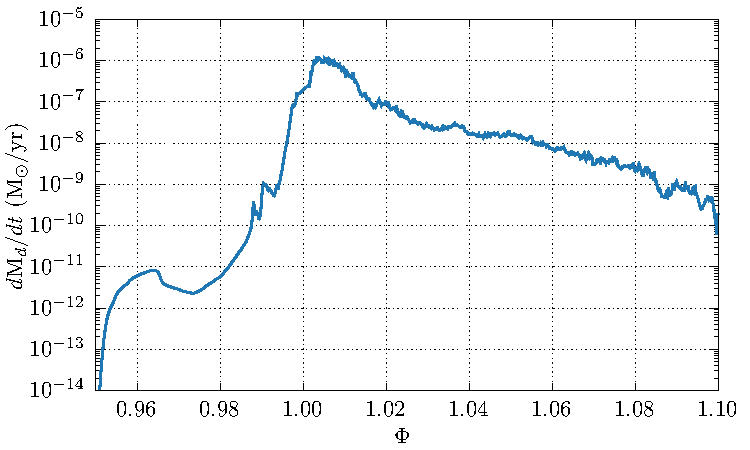
\includegraphics[width=\linewidth]{assets/wr140-dust_rate.pdf}
  \caption[A graph of the dust production rate in the WCR over the orbital phase $0.95 \leq \Phi \leq 1.10$]{A graph of the dust production rate in the WCR over the orbital phase $0.95 \leq \Phi \leq 1.10$. The dust production rate sharply increases as the stars pass their closest approach. Afterwards, the dust production rate begins to falter and slow, due to weaker wind collision effects via the separation distance and radial velocity.}
  \label{fig:wr140-dustproduction}
\end{figure}

\begin{figure}
  \centering
  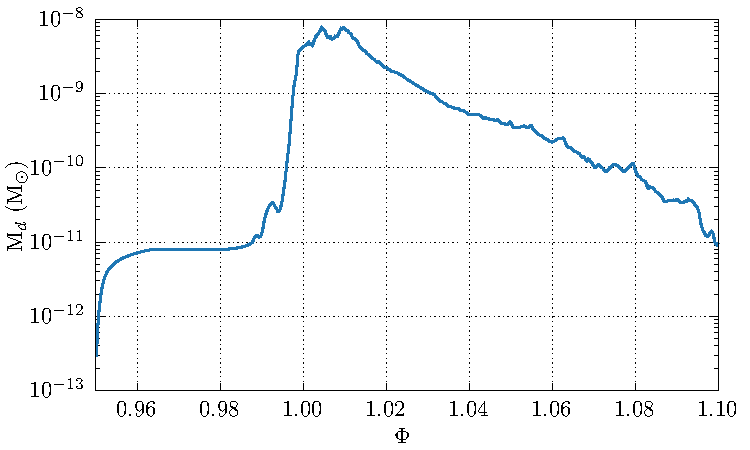
\includegraphics[width=\linewidth]{assets/wr140-m_dust.pdf}
  \caption[A graph of the overall dust mass in the simulation of WR140 over the orbital phase $0.95 \leq \Phi \leq 1.10$]{A graph of the overall dust mass in the simulation of WR140 over the orbital phase $0.95 \leq \Phi \leq 1.10$. The amount of dust quickly reduces after periastron due to a decreased dust growth rate (Fig. \ref{fig:wr140-dustproduction}), as well as dust advecting off the numerical grid.}
  \label{fig:wr140-dustmass}
\end{figure}

Dust growth was found to be consistent with previous uses of this particular dust model.
Dust production rates were found to be sensible, and below the theoretical maximum dust formation rate, $\mdot\rms{d,max} \approx \SI{4.8e-6}{\solarmass\per\year}$.
% Previous paper might be a bit of a whole thing, need to ask Julian how to reference to that
After an initial advection period lasting until $\Phi \approx 0.96$, the dust production rate rapidly increased as the stars approached periastron passage, peaking at $\Phi \sim 1.01$ (Fig. \ref{fig:wr140-dustproduction}).
This maximum dust production rate of \SI{1.24e-6}{\solarmass\per\year} is sensible, but incredibly prodigious.
We find peak conversion efficiency of gas into dust of $\sim 26\%$ in the WCR compared to the theoretical maximum dust production rate described in Eq. \ref{eq:p2-maxdustrate}, as well as a total conversion efficiency of $\sim 2.2\%$ throughout the entire system (assuming a total mass loss rate of \SI{5.76e-5}{\solarmass\per\year}).
The majority of dust production ($\gtrsim 90\%$) is produced within the WCR.
After reaching this maximum value, the dust production rate steadily decreases as the stars recede from each other.
This is reflected in the overall dust mass of the simulation (Fig. \ref{fig:wr140-dustmass}), as well as in infrared observations of WR140, where the infrared emission from dust formation rapidly reaches a maximum value after periastron passage, and slowly relaxes to a minimum value. % Find citation for this, plot
This asymmetry in the time-dependent change in infrared luminosity implies the existence of several factors for suppression and encouragement of dust formation than just the change in orbital separation distance.
It should be noted that due to the small size of the simulation, the dust mass in the system will reduce quickly, as dust advects off the numerical grid.

The evolution of dust in this system would result in the formation of an expanding cloud of dust every time the system passes periastron, with no contiguous spiral pattern forming, due to the lengthy ``dormant'' period occurring shortly after periastron passage.
This is consistent with observations of WR140, where these disconnected clouds are observed \citep{williams_orbitally_2009}.
We find an average dust production rate of $\mdot\rms{d} = \SI{7.68e-8}{\solarmass\per\year}$ over the entire simulation, and a change in the dust production rate by approximately five orders of magnitude over the course of the simulation.
This fits our understanding of an episodic dust forming WCd system, with an extremely clear ``active'' period followed by a slow tapering off of dust production as the system approaches the ``dormant'' period.
We can compare our results to the estimated dust yields from \cite{lauRevisitingImpactDust2020}, which found an average dust production rate of $\mdot\rms{d} = \SI{8.11e-10}{\solarmass\per\year}$ throughout an entire orbit of WR140.
Our value for the dust-to-gas mass ratio within the system appears to be sensible, while our average dust production rate is significantly higher.
This is due to the limited temporal sample of the simulation.
We would find a significantly lower average dust production rate over the course of a full orbit due to more sampling of the system over the ``dormant'' period.

\begin{figure*}
  \centering
  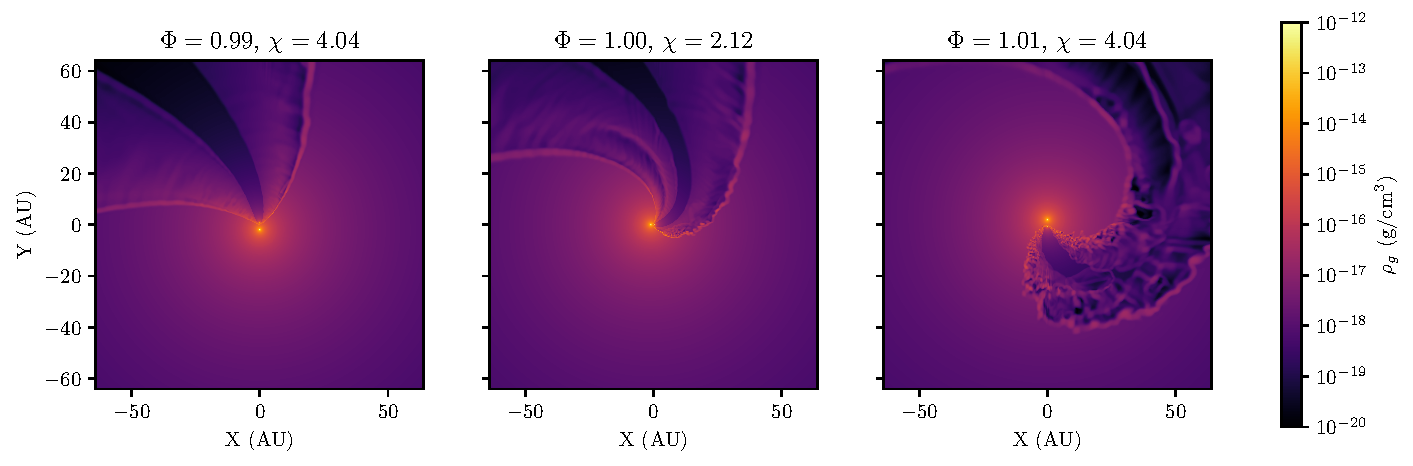
\includegraphics[width=0.95\linewidth]{assets/periastron-3-rho.pdf}
  \caption{Gas density in a simulation of the WR140 system shortly before, during, and after periastron. The value of $\chi$ is calculated using Eq. \ref{eq:p2-chi} and the WR wind parameter is noted in each panel. The simulation becomes dominated by instabilities after periastron. These instabilities persist despite the system behaving adiabatically at $\Phi = 0.99$, when the  orbital separation distance is identical. This suggests that the radiative behaviour of the post-shock WCR is due to other factors, in addition to $d\rms{sep}$.}
  \label{fig:p2-fullpage-rho}
\end{figure*}

\begin{figure*}
  \centering
  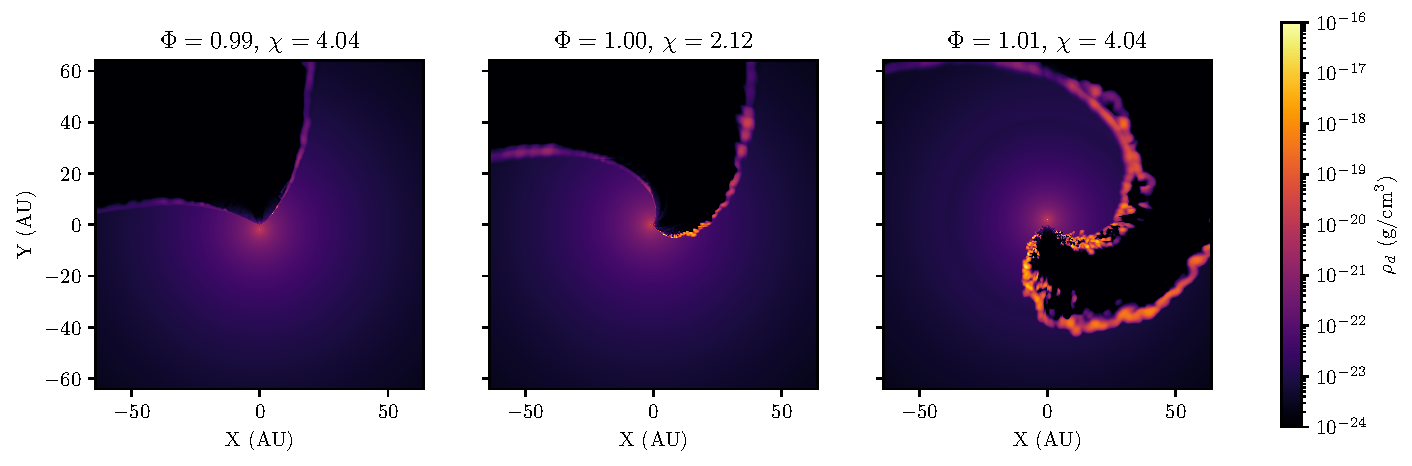
\includegraphics[width=0.95\linewidth]{assets/periastron-3-rhod.pdf}
  \caption{Dust density in a simulation of the WR140 system shortly before, during, and after periastron. Dust growth occurs as a direct result of the formation of cold, dense gas in the post-shock WCR.}
  \label{fig:p2-fullpage-rhod}
\end{figure*}

\begin{figure*}
  \centering
  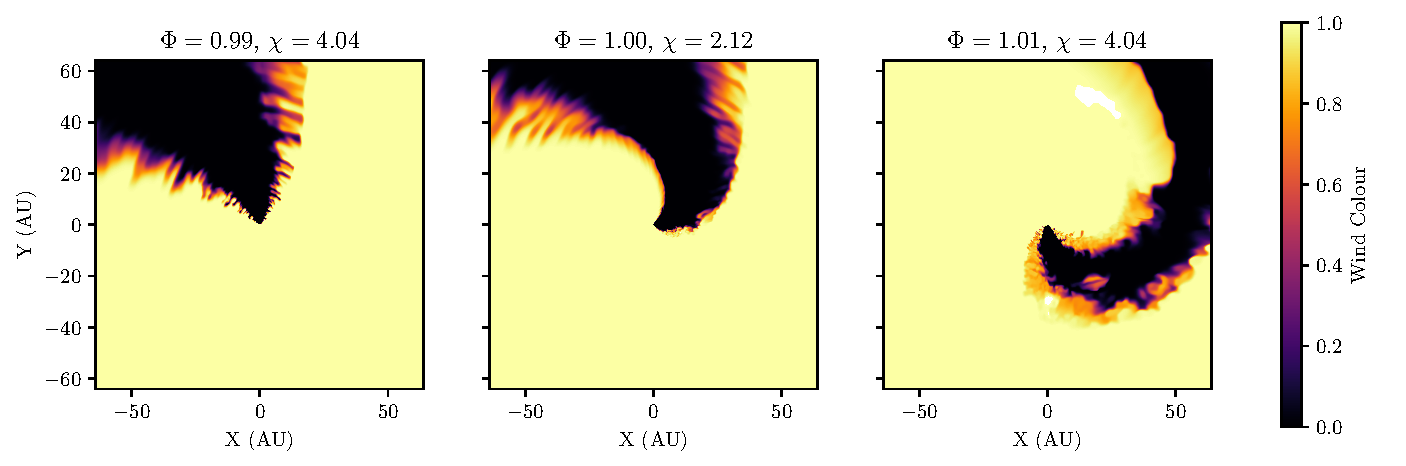
\includegraphics[width=0.95\linewidth]{assets/periastron-3-r0.pdf}
  \caption{Wind ``colour'' in a simulation of the WR140 system shortly before, during, and after periastron. A colour of 1 represents a pure WR wind and a colour of 0 represents a pure OB wind. We find that the wind undergoes more mixing during and after periastron.}
  \label{fig:p2-fullpage-r0}
\end{figure*}

\subsection{Instabilities}

% Instabilities

As can be seen in Fig. \ref{fig:p2-fullpage-rho}, after periastron passage the post-shock WCR region transitions from a smooth adiabatic wind to a highly radiative wind dominated by instabilities.
As the WCR becomes increasingly radiative, dust growth drastically increases, with the bulk of dust production occurring within the high density regions produced by these instabilities.
However these clumpy pockets of gas do not exhibit significant dust growth beyond $\sim \SI{20}{\au}$ from the simulation barycentre, with concentrations of dust remaining approximately constant (Fig. \ref{fig:p2-fullpage-rhod}).
% Induced instabilities, ie 
By the end of the simulation at $\Phi = 1.10$, the WCR is still somewhat dominated by instabilities, with an elevated dust production rate even though the cooling parameter has increased significantly to $\chi = 19.7$, which would normally imply adiabatic behaviour.
Whilst the dust production rate has reduced significantly, there is still a significantly greater growth rate than at the start of the simulation (after advection).
Clearly the transition from radiative back to adiabatic behaviour has a degree of latency, with instabilities still driving the structure of the WCR long after an adiabatic flow should have re-established.
Such behaviour was first reported by \cite{pittard_3d_2009} and leads to hysteresis in the x-ray emission \citep{pittard_3d_2010}.
This is the key physics responsible for the asymmetric dust growth rate about periastron.
It seems that once instabilities form in the WCR, they are somewhat difficult to stop - and cause oblique shocks, with lower post-shock temperature and ultimately stronger cooling than expected.
% Wind mixing
The amount of wind being mixed in the WCR also significantly increases after periastron passage, which would be conducive to the formation of complex organic molecules on the surface of the dust grains (Fig. \ref{fig:p2-fullpage-r0}).
Whilst this is beyond the scope of the current work, evolution of dust grains from WCd systems on longer time and length scales would be an enlightening avenue of research.

\subsection{Influence of varying wind velocity on dust production}

% Note change in dust yields from previous paper, will have to reference this when in publishing
As we have previously discussed, varying the wind terminal velocity for both stars in a simulation can result in significant changes in the dust production rate.
This is theorised to be due to the increased cooling in the WCR caused by slower winds, as well as through KH instabilities driven by a wind velocity shear (if the wind terminal velocities are significantly different, see \cite{stevens_colliding_1992}).
Previous work on this subject considered systems with circular orbits \textcolor{red}{\underline{\emph{\textbf{<<CITE EATSON ET AL. 2022 WHEN PUBLISHED>>}}}}, where the pre-shock velocities are constant over the orbit of the system.
However, in the case of a system with an eccentric orbit (such as WR140), the outflow velocity for each wind, as well as their ratio, can markedly vary over the systems orbit.
% Discuss change in relative velocity, will significantly impact, by as much as an order of magnitude? Write script to calculate change in chi?
As the stars approach periastron, the radial velocity, $v\rms{r}$, for each star rapidly changes from a maximum value to a minimum, as the stars approach and then swing past one another (Fig. \ref{fig:p2-shear}).
This causes a rapid change in the pre-shock velocity for both winds.
This then influences the amount of radiative cooling in the post-shock wind, suppressing radiative cooling pre-periastron and inciting it post-periastron; leading to changes in the dust production rate. 
While the change in wind velocity is relatively small (with the wind velocity varying by as much as 6\% over the course of an orbit) it still impacts the cooling of the system, and can vary $\chi$ by as much as a factor of 1.26 in the case of WR140.

% Velocity shear
The rate of dust production is also affected by the presence of a large wind velocity ratio, $\Upsilon$, where:

\begin{equation}
  \Upsilon = v\rms{OB} / v\rms{WR} .
\end{equation}

\noindent
As the mass of each star is different, the change in radial velocity differs for each star, causing a variability in the velocity ratio and therefore velocity shear.
Previous research with dust models suggests that a strong velocity shear drives an increased dust production rate.
We find that the maximum velocity shear occurs at $\Phi = 1.01$ (Fig. \ref{fig:p2-shear}), around the same time where the dust growth rate is at a maximum; this is consistent with our previous work.
% Whilst this will not dominate the dynamics of dust formation as a whole, this would explain asymmetry in dust formation rate curve
This change in velocity shear may therefore be another factor behind the increased dust growth of WR140 post-periastron.

We also note that in reality there could be significant change in the pre-shock velocity of the O wind due to the WCR encroaching into the acceleration region during periastron \citep{sugawaraSuzakuMonitoringWolf2015}.

% and explain why the system is still dominated by instabilities even after the system should be behaving adiabatically.
% However, this effect may also be decreased somewhat by the effect of radiative inhibition and braking on the winds.
% We find using a model estimating wind velocities using the \cite*{castor_radiation-driven_1975} model for radiative driving that the OB wind in particular is affected.
% Fig. \ref{fig:p2-cak} shows the wind velocities resultant from this model with CAK parameters for the WR and OB stars in WR140.
% We find that the wind velocity is approximately 84\% of the expected velocity.
% This would decrease the velocity shear before and after periastron passage.
% % reducing the velocity ratio on average, and resulting in a weaker velocity shear.
% The effect of radiative line driving from the CAK model is not considered in this simulation, and simulations considering this effect would have to be performed in order to study this further.
% This represents another interesting avenue of future research.



% \begin{figure}
%   \centering
%   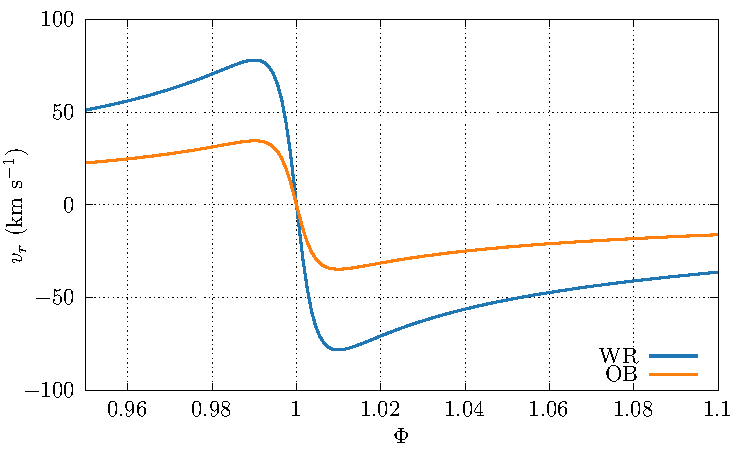
\includegraphics[width=\linewidth]{assets/radial-velocity/radial.pdf}
%   \caption[Radial velocity]{Radial velocity as a function of the orbital phase for the WR and OB stars in the WR140 system relative to the barycentre. As periastron passage occurs, the sudden inversion from approaching to receding can alter the wind velocity of the WR star by as much as \SI{160}{\kilo\metre\per\second}. Whilst this discrepancy is $\sim 6\%$ of the WR wind velocity, this can significantly increase dust production if the stars are receding from each other.}
% \end{figure}

\begin{figure}
  \centering
  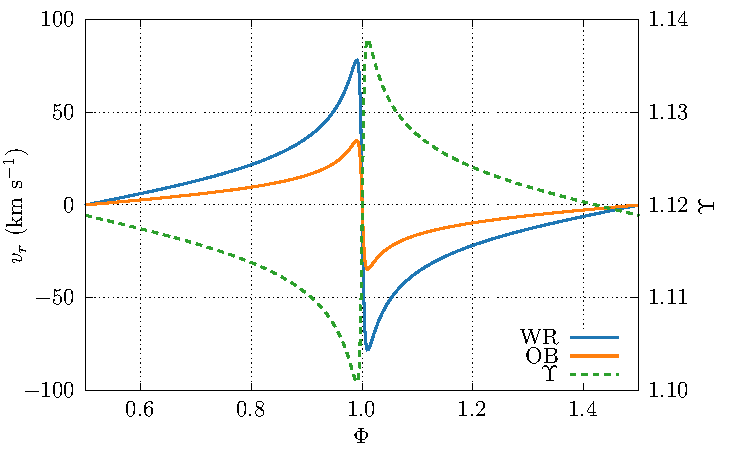
\includegraphics[width=\linewidth]{assets/radial-velocity/radial-shear.pdf}
  \caption[Radial velocity as a function of the orbital phase for the WR and OB stars in the WR140 system]{Radial velocity as a function of the orbital phase for the WR and OB stars in the WR140 system relative to the barycentre. As periastron passage occurs, the sudden inversion from approaching to receding can alter pre-shock the wind velocity of the WR star by as much as \SI{160}{\kilo\metre\per\second}. Whilst this is $\sim 6\%$ of the WR wind velocity, it can significantly increase dust production when the stars recede from each other. The velocity shear, $\Gamma = v\rms{OB}/v\rms{WR}$, also sharply increases during periastron passage, peaking at the point of maximum dust production.}
  \label{fig:p2-shear}
\end{figure}

% \begin{figure}
%   \centering
%   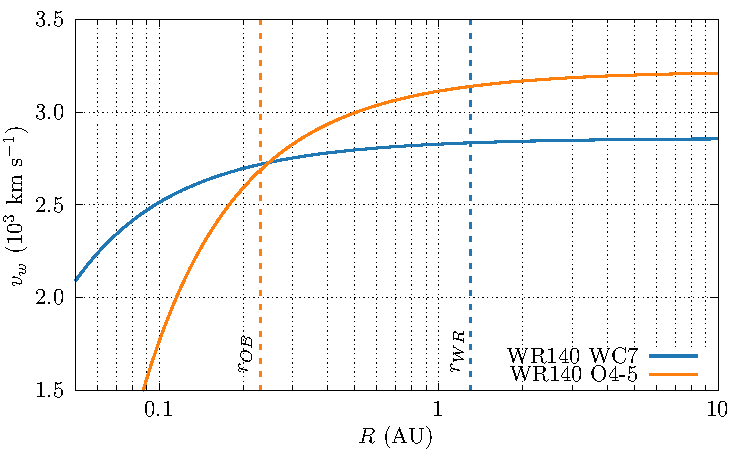
\includegraphics[width=\linewidth]{assets/stag.pdf}
%   \caption{Graph of the wind velocity of the WC7 and O4-5 stars in the WR140 system as a function of distance from the stellar surface due to radiative line driving. The dashed lines represent the distance to the WCR at periastron for each star. During periastron passage the WC7 wind is travelling at approximately its terminal velocity before collision, while the O4-5 companions wind is travelling at $\sim 84\%$ of terminal velocity before coming into contact with the WCR. CAK parameters were estimated to be $k = 0.37$, $\alpha = 0.60$ for the O4-5 star and $k=0.48$, $\alpha = 0.57$ for the WC7 star.}
%   \label{fig:p2-cak}
% \end{figure}


\section{Summary}
\label{sec:p2-conclusion}

Despite only simulating a limited section of the orbit of WR140, we have made a number of insights into the behaviour of the system.
We find a significant degree of change in the dust production rate as a direct consequence of the changing orbital separation of the system.
This is related to the change in the behaviour of the post-shock WCR wind, which goes from a smooth adiabatic wind to a clumpy, high density wind dominated by instabilities ideal for dust growth.
It is particularly interesting to note that the system does not revert to behaving adiabatically as quickly as expected.
This suggests that the post-shock WCR condition of the system is dependent on additional factors, instead of being solely due to $d\rms{sep}$.
One of the factors on this delayed return to the adiabatic state is potentially due to the orbital motion of the stars themselves.
As the stars approach each other at periastron, the radial velocity of the stars adds velocity to the wind beyond the outflow velocity, resulting in higher wind collision velocities, which encourages adiabatic behaviour in the post-shock flow.
The inverse is true as the stars recede from one another: the effective wind velocity for both stars is reduced, which encourages cooling and the formation of instabilities in the WCR.
Furthermore, an increased wind velocity ratio occurs after periastron due to the orbital dynamics which can drive KH instabilities.

% There is much additional research potential in simulating dust growth in episodic WCd systems.
% Further simulations of this system in particular would involve simulating a full orbit, through the use of AMR and increased computing time.
% Other avenues of research include the effect on dust formation due to the influence of radiative line driving and sudden braking, as well as a more complex, multi-fluid dust model where dust grains are not explicitly coupled to the stellar wind.

\section{Acknowledgements}

This work was undertaken on ARC4, part of the High Performance Computing facilities at the University of Leeds, UK.
We would also like to thank P. A. Crowther for his work on the Galactic Wolf-Rayet Catalogue (\url{pacrowther.staff.shef.ac.uk/WRcat}).

%%%%%%%%%%%%%%%%%%%% REFERENCES %%%%%%%%%%%%%%%%%%


\bibliographystyle{mnras}
\bibliography{references.bib} % if your bibtex file is called example.bib

% Don't change these lines
\bsp	% typesetting comment
\label{lastpage}
\end{document}

% End of mnras_template.tex
